\section{D. 가장 큰 정사각형}

\begin{frame} % No title at first slide
    \sectiontitle{D}{가장 큰 정사각형}
    \sectionmeta{
        \texttt{dynamic\_programming}\\
        출제진 의도 -- \textbf{\color{acsilver}Medium}
    }
    \begin{itemize}
        \item 출제자: \texttt{aru0504}
    \end{itemize}
\end{frame}

\begin{frame}{\textbf{D}. 가장 큰 정사각형}
    \begin{center}
        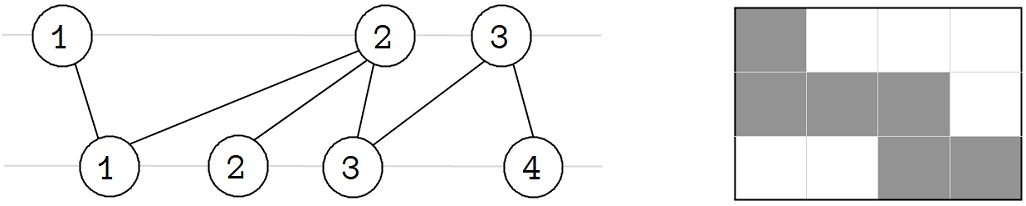
\includegraphics[width=0.8\linewidth]{../images/cow-fly/D-1.png}
    \end{center}
    \begin{itemize}
        \item $N \times M$ 격자를 그려봅시다.
        \item 위쪽 $i$번째 헛간과 아래쪽 $j$번째 헛간을 연결하는 항로가 있다면 격자의 $i$행 $j$열을 칠해줍시다.
        \item 놀랍게도 1행 1열에서 $N$행 $M$열까지 가는 최단경로 형태가 됩니다.
    \end{itemize}
\end{frame}